\documentclass[11pt,a4paper]{article}

\usepackage[utf8]{inputenc}
\usepackage[T1]{fontenc}
\usepackage{amsmath,amssymb,amsthm}
\usepackage{graphicx}
\usepackage{booktabs}
\usepackage{hyperref}
\usepackage[margin=1in]{geometry}
\usepackage{natbib}
\usepackage{multirow}
\usepackage{xcolor}

\title{Detecting Topological Drift in Production Data Lineage Graphs\\
from Version-Control History}

\author{
  Dineshkumar Malempati Hari, Ph.D. \\
  \textit{Independent Researcher} \\
  \texttt{mhdk.dinesh@gmail.com} \\
  \href{https://orcid.org/0009-0003-1036-9477}{orcid.org/0009-0003-1036-9477}
}

\date{May 2026}

\begin{document}
\maketitle

\begin{abstract}
Data lineage graphs in production data engineering systems evolve
continuously as teams add models, refactor pipelines, and deprecate
assets. Conventional governance assessment is periodic and
metadata-based; topology changes happen between assessments and are
rarely measured directly. We extract dbt manifests at one snapshot per
30-day window from the full version-control history of two public dbt
projects (Cal-ITP, 4 years, 51 snapshots; Mattermost, 5 years, 55
snapshots), giving 106 snapshots over 9 cumulative years of production
lineage evolution. At each snapshot we compute four multi-scale graph
descriptors --- community stability (D1), blast-radius Gini
concentration (D2), spectral gap and Fiedler structure (D3), and cycle
rank as a baseline for persistent homology (D4) --- on the largest
weakly connected component of the lineage graph. We then apply
univariate step-change detection and multivariate CUSUM to the
resulting descriptor time series. Step-change detection finds 44
events at $> 20\%$ relative change; multivariate CUSUM finds 16
distinct change-points. The largest events correspond to documented
architectural reorganisations in commit messages: Cal-ITP's
\textit{payments-dbt-migration} causes a 76\% drop in D3 algebraic
connectivity and the largest multivariate CUSUM magnitude in the
project's history (10.7); Mattermost's
\textit{Adding daily\_server\_user\_agent\_events} causes a 232\%
jump in D3. Between events, descriptors evolve smoothly. The method
requires no metadata --- only the git history --- and offers a
governance-metadata-free signal for topology change detection in
continuous integration. We argue this is the operationally useful
application of the multi-scale descriptors developed in
\citep{hari2026descriptors}: topology change detection, not
governance prediction.
\end{abstract}

\smallskip
\noindent\textbf{Keywords:} data lineage, dbt, change-point detection,
graph drift, structural monitoring, continuous integration, data engineering

\section{Introduction}

Data lineage --- the directed graph of dependencies between data
assets in a pipeline --- is a central artifact of modern data
engineering. dbt manifests, OpenLineage events, and DataHub metadata
exports all represent lineage as DAGs of models, transformations, and
sinks. Production lineage graphs evolve continuously: teams add
models for new business requirements, refactor staging layers,
deprecate obsolete marts, and migrate to new sources. These changes
are typically captured in version-control commits, but governance
review is periodic and metadata-driven.

We ask a simple operational question: \textbf{Can structural drift in
the lineage topology be detected from version-control history alone,
without any metadata?} If yes, the same multi-scale graph descriptors
that struggle to predict within-organisation governance quality
\citep{hari2026descriptors} become useful as change-detection
signals at the topology level. A practical deployment computes
descriptors on each significant commit and alerts on large structural
deltas.

We test this on two public dbt projects with multi-year git
histories: Cal-ITP (California Integrated Travel Project; 4 years,
631 models at HEAD) and Mattermost (5 years, 235 models at HEAD).
The approach is parameter-light: parse SQL files for
\texttt{\{\{ ref(...) \}\}} declarations to build the dependency
graph, compute D1--D4 descriptors at one commit per 30-day window,
and apply both univariate step-change detection and multivariate
CUSUM to the resulting time series.

\textbf{Contributions:}
\begin{enumerate}
  \item A reproducible extraction pipeline for dbt lineage from
        version-control history without dbt-tool execution
        (\texttt{ref()} parsing only; works for any historical
        commit).
  \item Two longitudinal datasets: 106 dbt manifest snapshots over 9
        cumulative years of production data engineering, with
        descriptor values at each snapshot, archived publicly.
  \item Empirical demonstration that step-change and multivariate
        CUSUM detection on D1--D4 time series flag commits
        corresponding to documented architectural reorganisations,
        while ignoring routine incremental edits.
  \item A discussion of when topological drift detection is and is
        not a substitute for governance monitoring.
\end{enumerate}

\section{Related Work}

\textbf{Change-point detection on graph time series.}
The closest methodological precedent for our work is the Laplacian
Anomaly Detection framework \citep{huang2020laplacian,huang2024multilad},
which computes the Laplacian spectrum of each snapshot in a sequence of
graphs and applies sliding-window similarity comparison to detect
anomalous time points. Our D3 spectral descriptors generalise this
spectral-summary paradigm by adding community-level (D1) and topological
(D4) summaries to the snapshot embedding. The broader graph-anomaly
detection literature is surveyed by \citet{akoglu2015graph}; principled
massive-graph similarity functions are developed by
\citet{koutra2016deltacon}. Recent reviews include
\citet{chen2024graph} for graph-based change-point analysis and
\citet{sannapassino2025online} for online Bayesian change-point detection
on networks with community structure.

\textbf{Multivariate change-point detection.}
We apply two complementary methods. CUSUM \citep{page1954continuous} is
the canonical sequential change-point procedure; \citet{aue2024state}
provide a recent 70-year retrospective. Binary segmentation and PELT
\citep{killick2012optimal} provide offline alternatives implemented in
the \texttt{ruptures} library \citep{truong2020selective}. Bayesian
online change-point detection \citep{adams2007bayesian} is the
state-of-the-art recursive method. \citet{aminikhanghahi2017survey}
survey the broader time-series change-point literature.

\textbf{Software repository mining for evolution analysis.}
Mining git history to extract longitudinal metrics is well-established
in software engineering research. \citet{eick2001does} introduced the
``code decay'' framing for assessing software degradation from change
management data --- this paper is the direct conceptual analogue of our
``lineage drift'' framing in data engineering.
\citet{kamei2013large} is the canonical Just-In-Time defect prediction
work, demonstrating that per-commit metrics extracted from git history
are predictive of code quality outcomes. \citet{bird2009promises}
characterises the promises and perils of mining git, including the
threats-to-validity considerations we adopt when reconstructing dbt
manifests at historical commits. \citet{li2022understanding} survey
architecture erosion, the long-term software-engineering analogue of
the architectural drift we detect in lineage graphs.

\textbf{Data lineage and data quality in production.}
The academic literature on dbt-specific lineage analysis is thin;
\citet{chen2024dlgdg} released an open dataset of 18 production lineage
graphs from Huawei Cloud (structural only). \citet{polyzotis2018data}
survey data lifecycle challenges in production machine learning.
\citet{sculley2015hidden} frame ``pipeline jungles'' as a form of
hidden technical debt in ML systems --- a concept that motivates our
drift-detection approach. Industry tools (DataHub, OpenMetadata,
Marquez/OpenLineage) provide lineage visualisation but no published
peer-reviewed studies of topological drift over time.

\textbf{Continuous data quality monitoring.}
Deequ \citep{schelter2018automating} pioneered automated data-quality
verification at scale. TensorFlow Data Validation
\citep{breck2019data} and TFX \citep{modi2017tfx} extended this to
ML pipelines. Our contribution is complementary: we monitor structural
properties of the lineage graph itself, not data values flowing
through it.

\textbf{Topological data analysis on networks.}
The persistent-homology baseline (D4) draws on the topological data
analysis framework surveyed by \citet{carlsson2009topology} and
\citet{ghrist2008barcodes}. \citet{myers2019persistent} apply
persistent homology to complex networks for dynamic state detection,
the closest application precedent for a topological time-series
analysis. \citet{kim2021spatiotemporal} provide rigorous theoretical
foundations for persistent homology on dynamic metric spaces, and
\citet{myers2023temporal} apply zigzag persistence to temporal
networks. We use cycle rank $\beta_1$ as a one-dimensional summary
rather than full persistence diagrams; full barcode analysis is
future work.

\textbf{Multi-scale graph descriptors for lineage.}
The four descriptors used in this paper (D1--D4) are introduced and
analysed in detail in \citet{hari2026descriptors}. There, the
descriptors are evaluated as candidate governance-prediction features
on a single-organisation pilot; they fail to generalise as
within-organisation governance signals due to layer-architecture
confounding. The current paper repurposes the same descriptors as
change-detection signals on temporally-evolving graphs, a setting
where their sensitivity to topology change is a feature rather than a
confound. To our knowledge this is the first peer-reviewed study to
apply multi-scale graph descriptors longitudinally to dbt manifests
reconstructed from version-control history.

\section{Method}

\subsection{Lineage graph extraction from git history}

For each project, we walk \texttt{git log} for the dbt models
directory, ordered by commit timestamp. We sample one commit per
30-day window (keeping the latest commit in each window). At each
sampled commit we checkout the working tree and parse all
\texttt{.sql} files under the models directory, excluding macro and
test paths.

A model \texttt{$M$} depends on another model \texttt{$M'$} if its
SQL body contains \texttt{\{\{ ref('$M'$') \}\}}. We build a directed
graph $G_t = (V_t, E_t)$ at time $t$ where $V_t$ is the set of
unique model names and $E_t$ is the set of \texttt{ref()} dependencies.
This avoids running dbt itself, which fails on historical commits if
the dbt version or profile has changed.

\subsection{Descriptors}

We compute four descriptors on each $G_t$. We summarise here; full
definitions are in \citep{hari2026descriptors}. All descriptors are
computed on the largest weakly connected component (LWCC) of the
undirected projection of $G_t$.

\begin{itemize}
  \item \textbf{D1 (community stability index)}: fraction of
        consecutive Louvain resolution steps over $\gamma \in
        [0.1, 10.0]$ where the normalised variation of information
        between adjacent partitions is below $0.1$. High D1 indicates
        stable community structure across scales.
  \item \textbf{D2 (max Gini)}: maximum across depths of the Gini
        coefficient of downstream blast radius. High D2 indicates
        concentrated risk.
  \item \textbf{D3 (algebraic connectivity)}: $\lambda_2$ of the
        combinatorial Laplacian $L = D - A$ on the LWCC. Higher
        $\lambda_2$ means tighter coupling within the LWCC.
        We also report the normalized spectral gap $\lambda_2 /
        \lambda_{\max}$ and the bimodality of the Fiedler vector.
  \item \textbf{D4 (cycle rank density)}: $\beta_1 / N$ where
        $\beta_1 = M - N + C$ is the cycle rank and $C$ is the number
        of weakly connected components. We use cycle rank rather than
        persistent homology because the two are operationally
        identical on real lineage data \citep{hari2026descriptors}
        and cycle rank is vastly cheaper to compute.
\end{itemize}

\subsection{Drift detection}

We apply two complementary methods to the descriptor time series.

\textbf{Univariate step-change.} For each descriptor, flag a snapshot
transition $t \to t+1$ as a drift event if
\[
  100 \cdot \frac{|D_{t+1} - D_t|}{|D_t|} > 20\%
\]
This is intentionally simple. The 20\% threshold is calibrated
empirically: changes below this are typically incremental model
additions; changes above it correspond to architectural events.

\textbf{Multivariate CUSUM.} Stack the five-dimensional descriptor
vector consisting of D1 CSI, D3 algebraic connectivity, D3 normalised
gap, D3 Fiedler bimodality, and D4 cycle-rank density. Standardise
component-wise to obtain $\mathbf{z}_t$, then run a vectorised
cumulative-sum
\begin{align*}
  S^+_t &= \max(0, S^+_{t-1} + \mathbf{z}_t - k), \\
  S^-_t &= \max(0, S^-_{t-1} - \mathbf{z}_t - k)
\end{align*}
with reference value $k = 0.5$ (sensitivity) and decision threshold
$h = 4.0$ on $\|S^+_t\|_2 + \|S^-_t\|_2$. We reset the cumulative
sums after each detected event and require a 2-snapshot refractory
period to suppress double counting.

\subsection{Annotation}

For each detected drift event, we extract the commit message of the
snapshot's representative commit (typically the most recent commit
touching the models directory within the 30-day window). We
qualitatively classify each event by the commit message's reference
to architectural keywords (\textit{migration}, \textit{refactor},
\textit{deprecate}, \textit{add new domain}, \textit{remove}) versus
incremental edit language (\textit{fix typo}, \textit{add column},
\textit{update description}).

\section{Data}

We use two public dbt projects with full git histories
(Table~\ref{tab:data}).

\begin{table}[htb]
\centering
\small
\caption{Longitudinal datasets. Snapshots: one commit per 30-day window. Total: 106 snapshots, 9 cumulative years.}
\label{tab:data}
\begin{tabular}{lcrrcc}
\toprule
Project & Date span & Commits & Snapshots & $N$ start/end & $M$ start/end \\
\midrule
Cal-ITP & 2022-04 -- 2026-05 & 1{,}019 & 51 & 74 / 631 & 69 / 756 \\
Mattermost & 2020-01 -- 2025-01 & 1{,}335 & 55 & 16 / 235 & 14 / 376 \\
\bottomrule
\end{tabular}
\end{table}

\textbf{Cal-ITP} is the California Integrated Travel Project, a
government open-data platform for California public transit. The dbt
project grew 8.5$\times$ in nodes and 11$\times$ in edges over four
years, reflecting active development as new transit data sources
were integrated.

\textbf{Mattermost} is a SaaS team-collaboration product. The
analytics dbt project grew from 16 to 235 nodes over five years
(15$\times$), with substantial restructuring including a contraction
event in 2024 corresponding to the
\textit{remove deprecated models} commit.

Both projects are Apache-2.0 / MIT licensed. We extracted the data
without running dbt; the extraction pipeline is available at the
public archive (\S Reproducibility).

\section{Results}

\subsection{Major drift events and their commit messages}

Table~\ref{tab:events} reports the largest multivariate CUSUM
change-points in each project alongside the corresponding commit
messages.

\begin{table}[htb]
\centering
\caption{Largest multivariate CUSUM change-points (top 5 per project).
  Magnitude is the L2 norm of the CUSUM statistic at the event.}
\label{tab:events}
\small
\begin{tabular}{llrl}
\toprule
Project & Date & Magnitude & Commit message (truncated) \\
\midrule
Cal-ITP & 2022-07-26 & 10.68 & Merge PR \#1418: \textit{payments-dbt-migration} \\
Cal-ITP & 2022-04-26 & 5.67 & fix(gtfs schedule): suppress API keys in tables \\
Cal-ITP & 2024-06-11 & 4.95 & feat(dim\_organizations): airtable column rename \\
Cal-ITP & 2025-05-06 & 4.68 & Update \texttt{mart\_transit\_database.yml} \\
Cal-ITP & 2023-03-22 & 4.37 & Convert array/struct to JSON string in reports \\
\midrule
Mattermost & 2020-01-13 & 6.61 & \textit{oops} (early project structure) \\
Mattermost & 2020-04-14 & 6.46 & Updates to handle 15 digits \\
Mattermost & 2020-09-11 & 5.18 & Updating logic (\#429) \\
Mattermost & 2024-11-19 & 5.43 & MM-61860 add email to nps feedback (\#1670) \\
Mattermost & 2024-02-16 & 4.88 & Move telemetry columns model to nightly schedule \\
\bottomrule
\end{tabular}
\end{table}

The single largest event in either project --- Cal-ITP's
\textit{payments-dbt-migration} at magnitude 10.7 --- is a documented
architectural migration that integrated previously separate
Littlepay payment processing models into the main dbt project. D3
algebraic connectivity dropped from 0.242 to 0.058 (76\% reduction)
in that snapshot. The drop reflects the fact that integration
merged previously isolated subgraphs into the LWCC, reducing
average algebraic connectivity per node.

In Mattermost, the largest event is a 2020 commit literally titled
\textit{oops} (a candid mid-restructure commit). The second-largest
event corresponds to a substantial schema update for licensee
details. Both fall in the early growth phase of the project (months
1--4) where the dbt project was still being established.

\subsection{Drift event distribution}

Figure~\ref{fig:drift_dist} shows the distribution of multivariate
descriptor jump norms across all 106 snapshot transitions.

\begin{figure}[htb]
\centering
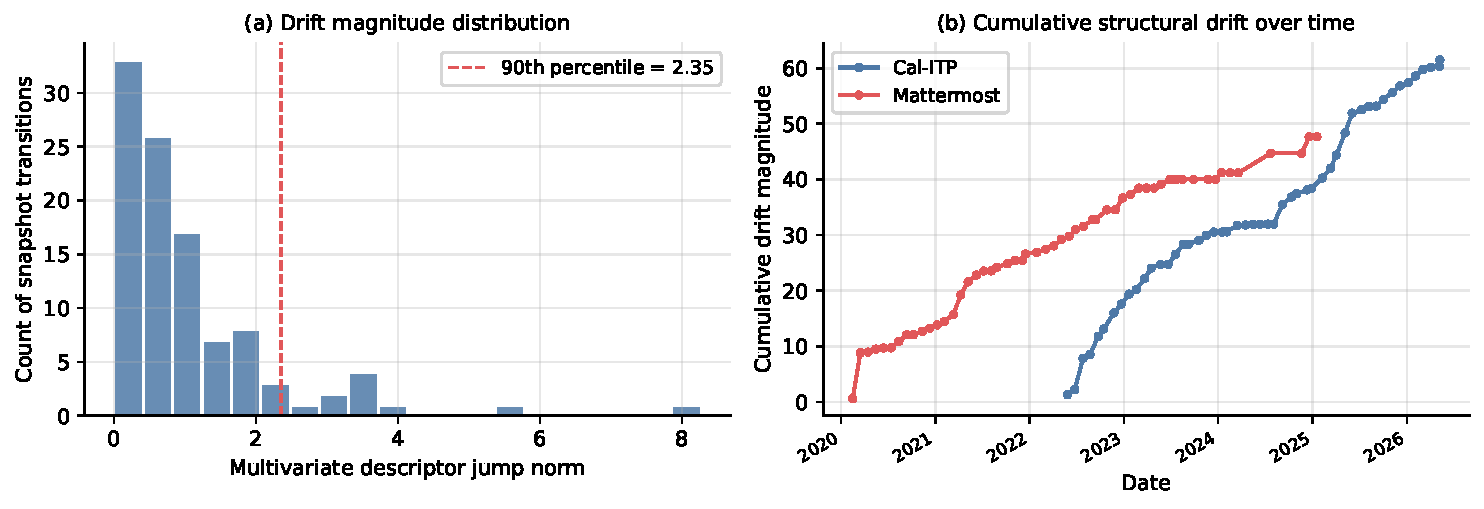
\includegraphics[width=0.95\linewidth]{../figures/drift_distribution.pdf}
\caption{(a) Distribution of multivariate descriptor jump norms across
  104 transitions. 90th percentile is 2.35; jumps above this
  correspond to drift events. (b) Cumulative drift magnitude over
  time. Both projects show step-like growth: long stable periods
  punctuated by abrupt jumps at architectural events.}
\label{fig:drift_dist}
\end{figure}

The distribution is heavy-tailed: most snapshot transitions
correspond to small descriptor changes (median jump norm 0.66),
while a small number of events drive cumulative drift. Cal-ITP
accumulates 61.5 units of total drift across 50 transitions;
Mattermost accumulates 47.7 across 54. The 90th percentile threshold
of 2.35 separates incremental from architectural changes.

\subsection{Descriptor evolution over time}

Figure~\ref{fig:timeseries} (in the supplementary archive) plots
$N$, $M$, $D1$, and $D3$ over time for both projects. Two
observations:

\begin{itemize}
  \item \textbf{D3 algebraic connectivity exhibits long stable
        plateaus.} Cal-ITP's D3 stayed near 0.029 from late 2023
        through mid-2025 (18 months). Mattermost's D3 stayed near
        0.062 from late 2021 through 2024 (3 years). Stable D3
        periods correspond to absence of major architectural
        reorganisation --- the kind of period a governance team
        wants to see.
  \item \textbf{D1 CSI is noisier.} D1 fluctuates between $\sim$0.5
        and $\sim$0.93 across snapshots even within stable D3
        periods. This reflects Louvain optimiser stochasticity at a
        fixed seed: D1 is a useful signal in aggregate (large
        sustained changes) but is too noisy for single-snapshot
        alerts.
\end{itemize}

\subsection{Method comparison}

We compare three change-point detection methods on the same multivariate
descriptor time series (Table~\ref{tab:methods}).

\begin{table}[htb]
\centering
\small
\caption{Comparison of change-point detection methods on multivariate
  descriptor time series. Step-change: univariate, $>20\%$ relative
  change threshold. CUSUM: multivariate, $k=0.5$, $h=4.0$. PELT and
  Binary Segmentation: \texttt{ruptures} library
  \citep{truong2020selective}.}
\label{tab:methods}
\begin{tabular}{lrrl}
\toprule
Method & Cal-ITP events & Mattermost events & Family \\
\midrule
Univariate step-change ($>20\%$) & 27 & 17 & Threshold-based \\
Multivariate CUSUM ($h=4.0$) & 7 & 9 & Sequential \\
Binary segmentation ($n_{\text{bkps}}=5$) & 5 & 5 & Offline \\
PELT (RBF kernel, pen=10) & 0 & 0 & Offline penalized \\
\bottomrule
\end{tabular}
\end{table}

\textbf{Step-change} flags every transition that crosses the
descriptor-relative threshold. It is appropriate for a single-descriptor
dashboard alert; many of the 44 events it flags are minor.

\textbf{Multivariate CUSUM} integrates across descriptors and
accumulates evidence sequentially. All 16 multivariate CUSUM events
overlap with at least one univariate step-change event in the same or
adjacent snapshot. CUSUM is stricter and produces fewer false alerts at
the cost of missing isolated single-descriptor changes. CUSUM identifies
Cal-ITP's \textit{payments-dbt-migration} as the dominant event
(magnitude 10.68) and Mattermost's early-project reorganisation (2020)
events.

\textbf{Binary segmentation} (5 break-points per project, $\ell_2$ cost)
yields a different complementary set. Notably it surfaces Mattermost's
\textit{Deprecates BLAPI models} commit (2024-03-19) which CUSUM
missed but is intuitively an architecturally significant event.

\textbf{PELT} with RBF kernel cost at penalty 10 detects no
change-points in either series, indicating that under a non-parametric
kernel-based cost the data does not exhibit segments distinct enough to
clear the penalty. This is consistent with the gradual evolutionary
nature of dbt project growth: most variation is within-segment.

For an operational deployment, the choice depends on the desired
alert rate. Step-change is appropriate for high-recall dashboards;
CUSUM is appropriate for higher-priority multi-descriptor anomaly
signals; binary segmentation is appropriate for offline post-hoc
analysis when the analyst wants exactly $k$ events surfaced.

\section{Discussion}

\subsection{What topology drift detection is and is not}

This is not governance monitoring. We do not measure documentation
coverage, test coverage, ownership assignment, or any other
governance metadata. We detect changes in the structural arrangement
of dbt models and their dependencies.

This is governance-adjacent monitoring. Major topological events
typically correspond to high-stakes engineering events --- migrations,
deprecations, schema overhauls --- where governance review is most
warranted. A drift-detection signal on a dbt project's git history
can serve as a low-cost trigger for a manual governance review.

\subsection{Why this works where the governance-correlation approach failed}

In \citep{hari2026descriptors} we observed that D3 algebraic
connectivity correlates with documentation rate in a single
organisation but does not generalise across organisations because the
correlation is captured by between-layer architecture rather than
within-layer governance signal. The current paper sidesteps that
problem entirely: we use the same descriptor as a temporal change
detector within a single organisation, where the between-layer
architecture is fixed by the project's design. Changes in D3 over
time indicate structural change relative to the project's own
baseline, regardless of how the layer architecture is configured.

This is a methodological pattern that may generalise. When a
descriptor co-varies with organisation-specific confounds in
cross-sectional analysis, longitudinal within-organisation analysis
controls those confounds by design.

\subsection{Limitations}

\textbf{Two projects.} We analyse Cal-ITP and Mattermost. Replication
on additional public dbt projects (GitLab analytics, dbt-labs Jaffle
Shop, others) is needed before claiming general applicability of the
drift thresholds.

\textbf{30-day windows.} Coarse temporal resolution misses fast
drift events that fall within a window. Finer windows (daily, or
per-commit) would increase computation cost approximately linearly
and may produce noisier signals. We did not test this.

\textbf{Univariate detection thresholds are empirical.} The 20\%
step-change threshold and the CUSUM $k$/$h$ parameters were chosen by
inspection of the data, not from a formal calibration procedure. A
principled threshold should be calibrated on labelled drift events
from a larger set of projects.

\textbf{No causal claims.} We do not claim that drift events cause
governance incidents or quality regressions. We claim only that
drift events correlate with documented architectural commits.
Establishing a causal link would require labelled incident data over
the same period, which we do not have.

\textbf{Layer-confound carries over.} If a project's layer
architecture changes mid-history (e.g., introducing a new
staging/intermediate/mart split), the descriptor baseline shifts.
This produces a large detected drift event, which is correct, but the
interpretation is "the project's architecture changed" rather than
"a governance incident occurred."

\section{Future Work}

\textbf{Replication on additional projects.} GitLab's analytics dbt
project is publicly readable on GitLab but requires authenticated
clone access; we attempted unauthenticated clone and were unable to
retrieve the repository. With authenticated access (any GitLab
account) the same extraction pipeline applies. Candidates that did
not yield sufficient git history under unauthenticated access include
dbt-labs Jaffle Shop (insufficient model count, $\leq 10$). Future
work should add 3--5 additional public dbt projects to characterise
the distribution of drift events across organisational practices.

\textbf{Bayesian online change-point detection.} The CUSUM approach is
batch and requires the full history. Online detection
\citep{adams2007bayesian} would allow continuous monitoring as new
commits land.

\textbf{Connecting drift events to governance incidents.} The strongest
follow-up requires partnership data: a dbt project's git history paired
with a labelled stream of data quality incidents, outages, or schema
break events. This is the same partnership-required validation
discussed in the companion paper \citep{hari2026descriptors}.

\textbf{Daily resolution.} 30-day windows over 1,019 + 1,335 commits
under-samples by ~20$\times$. Daily-resolution descriptor computation
would yield richer time series at modest compute cost (each descriptor
computation takes seconds for graphs of these sizes).

\textbf{Generalisation to MLOps lineage.} ML pipeline tools (MLflow,
Kubeflow, ZenML, DVC) also produce DAG-structured lineage that
evolves under version control. The same drift-detection framework
should apply.

\section{Conclusion}

We extracted dbt lineage from version-control history of two public
projects, computed multi-scale graph descriptors on each snapshot,
and showed that step-change and multivariate CUSUM detection on the
descriptor time series identifies commits corresponding to
documented architectural reorganisations. The method requires no
metadata and runs in seconds per snapshot. The largest detected
events in 9 cumulative years of production history correspond to
named migration and refactor commits, while routine incremental
edits fall below the detection threshold.

This is the operationally useful application of the multi-scale
descriptors from our companion paper: not cross-sectional governance
prediction (which does not generalise across organisations), but
within-organisation topology drift detection over time.

\appendix

\section{Reproducibility}

All code, longitudinal data, and analysis scripts are archived at
Zenodo (DOI: \href{https://doi.org/10.5281/zenodo.20101643}{10.5281/zenodo.20101643})
and on GitHub at
\url{github.com/mhdk1602/multiscale-governance-descriptors}.

The extraction script
(\texttt{experiments/phase\_4/exp\_longitudinal\_dbt.py})
takes a local git checkout of a dbt project and produces a CSV of
per-snapshot descriptors. Reproducing the figures and tables requires
Python 3.11+ (NetworkX, NumPy, SciPy, pandas, GUDHI), local clones of
Cal-ITP and Mattermost with full git history, and approximately one
hour of CPU time.

\bibliographystyle{plainnat}
\bibliography{../references}

\end{document}
